%
% teil5.tex
%
% (c) 2023 Vincent Haufe, Hochschule Rapperswil
%
% !TEX root = ../../buch.tex
% !TEX encoding = UTF-8

\section{Weitere Anwendungen des Faltungstheorems auf $\mathbb{R^+}$
\label{mellin:section:teil5}}
\rhead{Teil 5}
Dieser letzte Abschnitt soll einen kurzen Einblick in einen 
weiteren Anwendungszweck der Mellin-Transformation geben und 
beruht auf\cite{mellin:mellin-transform-method}.
Darin findet sich eine umfangreiche Behandlung der 
Mellin-Transformation-Methode, sowie weitere Beispiele 
von Problemen in der Antennentechnik, für welche die Methode 
Anwendung findet.
Bisher haben wir diese als Möglichkeit kennengelernt, ein 
bestimmtes Registrierungsproblem numerisch effizienter zu lösen.
In dieser zweiten Anwendung geht es darum, gewisse, sonst schwierig 
zu lösende Integrale, die bei technischen Berechnungen auftreten 
können, mithilfe des Faltungstheorems der Mellin-Transformation 
analytisch weiter zu vereinfachen.
Das bietet in gewissen Fällen eine bessere Ausgangslage für weitere 
numerische oder analytische Berechnungen mit mathematischer Software 
wie {\em Mathematica}, als wenn diese sofort numerisch ausgewertet 
werden würden.
Ebenfalls bleiben bei einer analytischen Auswertung die physikalischen 
Zusammenhänge der Parameter erhalten, was zu einem besseren Verständnis 
derselben führen kann.

\subsection{Mellin-Transformation-Methode
\label{mellin:subsection:mtmethod}}
Die Mellin-Transformation-Methode ist ein analytisches Werkzeug 
zur Umformung eindimensionaler, endlicher Integrale.
Ihre Anwendung benötigt Kenntnisse der komplexen Analysis, da 
die Mellin-Transformierte wichtiger Funktionen meist in Form von 
$\Gamma$-Funktionen erscheint, wie sich der Tabelle \ref{fig:mellin:tabelle} 
entnehmen lässt.
\begin{figure}
    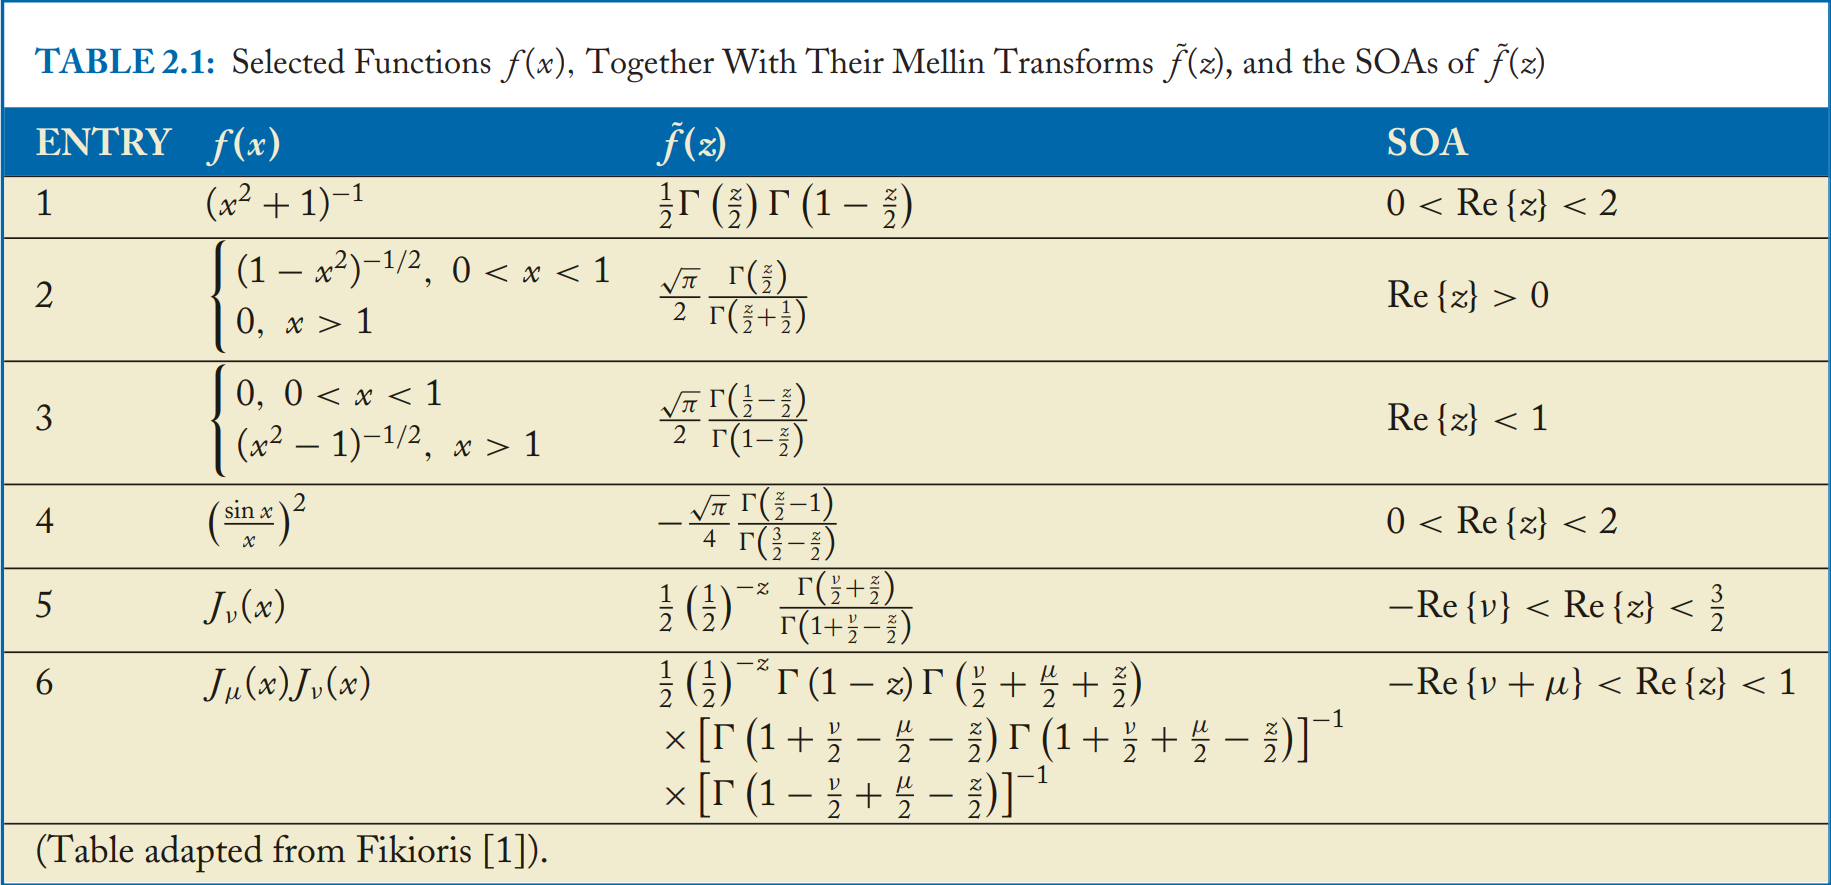
\includegraphics[width=\textwidth]{papers/mellin/images/mellin_tabelle.png}
    \caption{Einige Transformationspaare der Mellin-Transformation 
    (Aus \cite{mellin:mellin-transform-method})}
    \label{fig:mellin:tabelle}
\end{figure}
% legal?
Die $\Gamma$-Funktion ist dabei die Mellin-Transformierte der Funktion 
$f(x)=e^{-x}$.
\begin{equation}
    \Gamma(z) = 
    \int_{0}^{\infty} x^{z-1}e^{-x} \,dx,
    \qquad \operatorname{Re}(z) > 0
\end{equation}
Sie ist aber nicht nur im Kontext der Mellin-Transformation relevant, 
sondern auch in vielen anderen Bereichen der komplexen Analysis.
Dieses Thema soll hier allerdings nicht weiter aufgegriffen werden, 
und stattdessen mehr das Konzept der Methode aufgezeigt werden.

Der Kern der Methode ist hier wieder das Faltungstheorem.
\[
    (f \ast g)(x) 
    = \mathcal{M}^{-1}(\hat{f}(z) \cdot \hat{g}(z))(x)
\]
% \begin{align*}
%     (f \ast g)(x) &= \mathcal{M}^{-1}(\hat{f}(z) \cdot \hat{g}(z))(x) \\
%     f(x) \cdot g(x) &= \mathcal{M}^{-1}((\hat{f} \ast \hat{g})(z))(x)
% \end{align*}
Das Ziel ist es nun, das zu analysierende Integral in 
eine Form zu bringen, die einer multiplikativen Faltung entspricht.
Über das Faltungstheorem kann das Integral anschliessend ausgedrückt 
werden, als Rücktransformation des Produktes der Mellin-Transformierten, 
was eben konkret zu einem Integral über das Produkt von  
$\Gamma$-Funktionen führt, welche mittels Reihenentwicklung analytisch 
relativ gut weiter zu verarbeiten sind.

\subsubsection{Beispiel der Mellin-Transformations-Methode}
Folgender Ausschnitt einer Anwendung aus\cite{mellin:mellin-transform-method} 
soll die Methode demonstrieren.

In der Anwendung geht es um die Berechnung einer 
kreisförmigen Rahmenantenne\footnote{engl. circular, thin-wire loop antenna}.
Ein Ausdruck für das elektrische Feld $E_\phi $ wird über das Vektorpotential 
der Schleife aufgestellt.
Aufgrund der geometrischen Gegebenheiten enthält dieser die Bessel-Funktion $J_1$.
\[
    E_\phi 
    = -\zeta_0 H_\theta  
    = \frac{I_0ka\zeta_0e^{-jkr}}{2r} J_1(ka \sin\theta)
\]
Die abgestrahlte Leistung folgt über das Hüllflachenintegral über eine Sphäre.
Um aber nicht nur die abgestrahlte Leistung, sondern auch die Direktivität und 
den Strahlungswiderstand $R_r$ im Zuge des {\em cavity model} zu bestimmen, 
wird eine verallgemeinerte Version des Integrals aufgestellt
\[
    f(x, \mu, \nu, \tau)
    = \int_{0}^{\pi/2} J_\mu(x \sin\theta) J_\nu(x \sin\theta) 
    \sin^\tau \theta \,d\theta, \qquad x > 0 
    ,
\]
wobei im Falle der kreisförmigen Rahmenantenne $\mu = \nu = \tau = 1$ ist.
Die Funktion $f(x, \mu, \nu, \tau)$ lässt sich aber mithilfe der Theorie 
der Mellin-Transformation weiter analysieren.
Es wird die Substitution
\[
    \sin\theta = y
\]
durchgeführt.
Das führt auf den Ausdruck
\[
    f(x, \mu, \nu, \tau)
    = \int_{0}^{1} \frac{J_\mu(xy) J_\nu(xy)}{\sqrt{1-y^2}} y^\tau \,dy, 
    \qquad x > 0 
    .
\]
Um die Konvergenz des Integrals sicherzustellen, wird angenommen, dass
\[
    \operatorname{Re}(\mu) > 0,
    \operatorname{Re}(\nu) > 0,
    \operatorname{Re}(\tau) > 0.
\]
Die Substitution hat das Integral nun in eine sehr interessante Form gebracht.
Definiert man die Funktionen 
\begin{align*}
    g(x) &= J_\mu(x)J_\nu(x), \\
    h(x) &= \frac{x^\tau}{\sqrt{1-x^2}} 
\end{align*}
und ersetzt damit den Inhalt des Integrals, erscheint
\[
    f(x, \mu, \nu, \tau)
    = \int_{0}^{1} g(xy) h(y) \,dy, 
\]
was der multiplikativen Korrelation der beiden Funktionen entspricht!
Das bedeutet, dass die Funktion $f(x, \mu, \nu, \tau)$ sich als 
Rücktransformation des Produktes der Mellin-Transformierten $\hat{g}$ 
und $\hat{h}$ darstellen lässt.
Das Resultat dieser Rechnung führt auf die Zerlegung 
\begin{align*}
    f(x, \mu, \nu, \tau)
    = &\frac{\sqrt{\pi}}{4} \frac{1}{2\pi j} 
    \int_{\delta -j\infty}^{\delta +j\infty} 
    \frac{\Gamma(1 - z)\Gamma(\frac{\nu}{2}+\frac{\mu}{2}+\frac{z}{2})}{\Gamma(1+\frac{\nu}{2}-\frac{\mu}{2}-\frac{z}{2}) \Gamma(1+\frac{\nu}{2}+\frac{\mu}{2}-\frac{z}{2})} \\
    &\cdot \frac{\Gamma(\frac{1}{2}-\frac{z}{2}+\frac{\tau}{2})}{\Gamma(1-\frac{\nu}{2}+\frac{\mu}{2}-\frac{z}{2})\Gamma(1-\frac{z}{2}+\frac{\tau}{2})} 
    \left(\frac{x}{2}\right)^{-z} \,dz,
    \qquad -\operatorname{Re}(\nu + \mu) < \delta < 1
    .
\end{align*}
Diese mag zwar zuerst einschüchternd und komplizierter wirken, lässt 
sich aber mithilfe der komplexen Analysis gut weiterverarbeiten.

Für die Rahmenantenne ergibt sich daraufhin eine neue analytische 
Approximation für den Strahlungsiderstand 
\[
    R_r \sim 60\pi^2 \frac{C}{\lambda}
    \left[1+\frac{1}{\sqrt{\pi}}\left(\frac{C}{\lambda}\right)^{-1/2} 
    \cos\left(2\frac{C}{\lambda}+\frac{\pi}{4}\right)\right] \Omega
    ,
\]
die sehr nahe an die numerische Berechnungen der Funktion $f(x, \mu, \nu, \tau)$ 
herankommt, nun aber zusätzlich die physikalischen Zusammenhänge der 
Parameter offenbart.
\medskip

Tatsächlich ist die Mellin-Transformation-Methode bereits Teil der  
modernen symbolischen Integrationsroutinen von {\em Mathematica}.
Ein Verständnis der Methodik dieser Integrationsroutinen kann aber
allenfalls von Nutzen sein.
% Eine umfangreiche Behandlung der in diesem Abschnitt nur kurz 
% vorgestellten Mellin-Transformation-Methode, sowie weitere 
% Beispiele von Problemen in der Antennentechnik für welche die 
% Methode Anwendung findet, findet sich im 
% gleichnamigen Buch\cite{mellin:mellin-transform-method}.


% Einstieg, Anwendung führt in KomA (oder symbolic integration routines, software), weitere Analyse in Gelfandtheorie (the Beyond)
%     Gamma-Funktion
%     Mellin-Barnes
% kleine Horizonterweiterung